% hidelinks
% \documentclass[12pt,a4paper,twoside,openright]{scrreprt}
\documentclass[12pt,a4paper,twoside,openright]{report}

% basics
\usepackage[ngerman]{babel}
\usepackage[utf8]{inputenc}
\usepackage[T1]{fontenc}
\usepackage{cmap} % allow copy paste from pdf
\usepackage{graphicx}
\usepackage{minted}
\usepackage[babel]{microtype}
\usepackage{mathtools}
\usepackage[hyphens]{url}
\usepackage[unicode]{hyperref}
\usepackage[math]{blindtext}
\usepackage[mode=text,group-minimum-digits=4,round-mode=places,round-precision=2]{siunitx}

% \usepackage{tabularx}
% \usepackage{listings}
% \usepackage{algorithm}
% \usepackage{algpseudocode}
% \usepackage{amsmath}
% \usepackage{amssymb}
% \usepackage{listingsutf8}
% \usepackage{multirow}
% \usepackage{booktabs}
% \usepackage{longtable}
% \usepackage{float}
% \usepackage{caption}
% \usepackage{abstract}
% \usepackage{ccicons}
% \usepackage{tikz}
% \usepackage{tablefootnote}
% \usepackage{color}
% \usepackage{scrhack}
% \usepackage{array}
% \usepackage{fancyvrb}
% \usepackage{appendix}
% \usepackage[amsmath,hyperref]{ntheorem}

\usepackage[
    title={Implementierung einer parallelen Points-To Analyse},
    author={Lukas Böttcher},
    type=master,
    institute={Christian-Albrechts-Universität zu Kiel},
    course=cs,
    examiner={Prof.\ Dr.\ Hans Mustermann},
    supervisor={Dipl.-Inf.\ Roman Tiker,\\Dipl.-Inf.\ Laura Stern,\\Otto Normalverbraucher,\ M.Sc.},
    startdate={2022-08-01},
    enddate={2023-01-16},
    language=deutsch
]{scientific-thesis-cover}

% set up biblatex
\usepackage[
  backend       = biber,
  sortcites     = true,
  bibstyle      = alphabetic,
  citestyle     = alphabetic,
  giveninits    = true,
  useprefix     = false, %"von, van, etc." will be printed, too. See below.
  minnames      = 1,
  minalphanames = 3,
  maxalphanames = 4,
  maxbibnames   = 99,
  maxcitenames  = 2,
  natbib        = true,
  eprint        = true,
  url           = true,
  doi           = true,
  isbn          = true,
  backref       = true]{biblatex}
\bibliography{literatur}

% set up hyperref
\hypersetup{
    linktoc=all,
    bookmarksnumbered=true,
    bookmarksopen=true,
    bookmarksopenlevel=1,
    breaklinks=true,
    pdftitle={Masterarbeit},
    pdfstartview=Fit,
    pdfpagelayout=SinglePage,    
}


\begin{document}
\pagestyle{empty}
\Coverpage
\Affirmation
\cleardoublepage
\begin{abstract}
    \blindtext[1]
\end{abstract}
\cleardoublepage
\tableofcontents
\cleardoublepage
\listoffigures
\cleardoublepage
\listoftables
\cleardoublepage

\pagestyle{headings}
\blinddocument

\section{Test}

\begin{minted}[mathescape, linenos]{python}

    # Note: $\pi=\lim_{n\to\infty}\frac{P_n}{d}$
    title = "Hello World"
    
    sum = 0
    for i in range(10):
     sum += i
\end{minted}

\begin{figure}
    \centering
    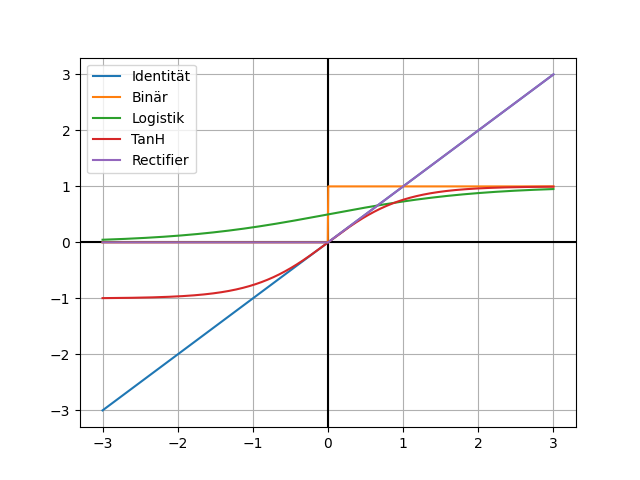
\includegraphics[width=0.8\textwidth]{img/test.png}
    \caption{Einige typische Aktivierungsfunktionen}
    \label{fig:actfn}
\end{figure}


\begin{table}[h!]
    \begin{center}
      \caption{More rows.}
      \label{tab:table1}
      \begin{tabular}{l|S|r}
        \textbf{Value 1} & \textbf{Value 2} & \textbf{Value 3}\\
        $\alpha$ & $\beta$ & $\gamma$ \\
        \hline
        1 & 1110.1 & a\\
        2 & 10.1 & b\\
        3 & 23.113231 & c\\
        4 & 25.113231 & d\\ % <-- added row here
      \end{tabular}
    \end{center}
  \end{table}

after minted
this works 
Objekte
\cite{juliani2018unity}

\blinddocument

\printbibliography[heading=bibintoc]
\end{document}